\documentclass[twocolumn]{article}

\usepackage{amssymb}
\usepackage{amsmath}
\usepackage{graphicx}
\usepackage{epstopdf}
\usepackage{fancyhdr}
\usepackage{algpseudocode}

\DeclareMathSizes{36}{36}{36}{36}

\title{Massively Parallel Ant Colony Optimization Applied to the Traveling Salesman Problem}
\author{Forest Trimble, Scott Todd\\trimbf@rpi.edu, todds@rpi.edu}

\begin{document}

\maketitle

\pagestyle{fancy}
\fancyhead{}
\fancyhead[L]{Trimble, Todd}
\fancyhead[C]{Massively Parallel ACO on the TSP}
\fancyhead[R]{\today}


\begin{abstract}
  \emph{NP-complete problems have often fascinated programmers and mathematicians alike
  for their difficulty, and the traveling salesman problem is no exception. We 
  study ant colony optimization, a naturally inspired optimization algorithm,
  as applied to the traveling salesman problem. We present an overview of
  the traveling salesman problem and the ant colony optimization algorithm before
  parallelizing it to run on the Blue Gene/Q and analyzing its performance. }
\end{abstract}

\section{Background} \label{sec:tsp}

The traveling salesman problem (TSP) is an extensively-studied NP-complete problem 
in theoretical computer science with varied applications throughout delivery, 
transportation, planning, and logistic operations. In the formulation of the 
problem, a list of cities is given and the distances between each pair of cities
is known. The question, then, is: what is the shortest possible path from city to
city that visits each city exactly once? In particular, we studied the symmetric
traveling salesman problem, where the distance from any city A to any city B
is the same as the distance from city B to city A. In this case, the problem
can be modeled as an undirected graph, with vertices representing cities and
edges representing paths between cities. For interests' sake, Figure \ref{fig:opt2392}
shows an optimal tour of 2392 cities in the undirected case. \\

\begin{figure}
  \centering
  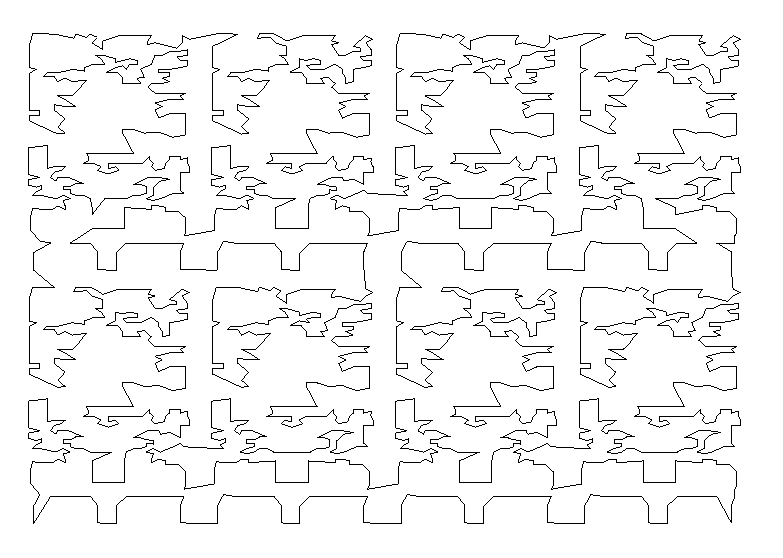
\includegraphics[height=2.2in]{plots/pr2392.eps}
  \caption{An Optimal TSP Tour of 2392 Cities} \label{fig:opt2392}
\end{figure}

The brute force approach to the TSP, which checks each possible solution, takes 
on the order of $\mathcal{O}(n!)$ time. Brute force is generally a pretty poor choice of
algorithm, and that is no different here: as it stands, the most efficient 
algorithms, which provably return the optimal solution, use dynamic
programming and operate in $\mathcal{O}(n^22^n)$ time and $\mathcal{O}(2^n)$ space. 
This is a massive time improvement, but it is still computationally intractable, as 
these large run-times and space requirements are prohibitively expensive even on 
supercomputer-class machines. Because of this, a large number of approximation 
algorithms have been formulated that are able to quickly approach the optimal 
solution, some provably within a certain threshold or with a high probability of
being particularly close to the optimal solution.  \\

The Ant Colony Optimization algorithm (ACO) for the Traveling salesman problem 
is one such approximation algorithm which lends itself well to parallel 
computation. It was first proposed by Marco Doringo's PhD thesis in 1992 \cite{dorigo}. 
Inspiration for this technique comes from the natural world, where ants in a
colony wander seemingly aimlessly until they come across food, leaving
a trail of pheromones for other ants to detect and follow. Pheromones
evaporate over time, so shorter paths accumulate pheromones in a higher density 
more reliably than longer paths. An emergent property of this behavior is that 
efficient paths to food sources will become apparent as more ants wander and 
follow these trails over time. Interestingly, the natural world provides a number
of such heuristics for optimization problems; the interested reader should 
refer to \cite{nature} for an overview of a few of them. \\

Just as these ants are able to find efficient routes to their food sources by
utilizing this emergent behavior, computers are able to find short paths through
graphs for the TSP by simulating ants and their pheromone trails. \\

An added advantage to the ACO, which is not explored here, is that
the virtual ants are able to adapt to changes in their environment to 
dynamically adjust their preferred path around newly introduced obstacles 
\cite{iridia:aco}.

\section{The Ant Colony Optimization Algorithm} \label{sec:aco}

It is important to understand how ACO works before diving into 
the implementation details. As such, this section delves
into the concepts behind ACO before covering the
specifics of the implementation in section \ref{sub:acoimpl} \\

Ant Colony Optimization is a randomized process that uses a few things to aid
in its probabilistic selection:
\begin{itemize}
\item distances between cities
\item pheromone concentrations along edges ($\tau$)
\item heuristic parameters $\alpha$, $\beta$, and $\rho$
\end{itemize}
Basically, shorter distances and higher pheromone concentrations will
increase the probability that an ant will travel along an edge. The 
heuristic parameters allow for some variation as to how important 
each of these factors is. This is necessary because an effective 
implementation of the ACO for TSP algorithm must balance the tendency
for ants to follow efficient paths with the desire to discover new, 
perhaps more efficient paths. If the simulated ants follow the 
pheromone trails too closely, they may quickly get caught in local
minima. \\

The heuristic parameters $\alpha$ and $\beta$ are weights for the distances and 
the pheromones, respectively, and they can be chosen to help avoid this. They 
are used to calculate the probability, $p^k_{ij}$, of an ant following an edge
$ij$ at iteration $k$ according to 
\begin{equation}
p_{ij}^k = \frac{(\tau^k_{ij})^\alpha(d(C_i,C_j)^-\beta)}{\sum_{i=1}^m 
  (\tau^k_{ij})^\alpha(d(C_i,C_j)^{-\beta})} \label{eq:probs}
\end{equation}
Thus, if $\alpha >> \beta$, the pheromones will factor in far more than the
distances. When $\beta >> \alpha$, the same is true only if the distances are 
normalized to the range $[0,1]$; otherwise $\|\beta\|$ is effective only in 
weeding out the larger distances. Some researchers have experimented with 
updating the heuristic parameters as the algorithm executes \cite{ipcsit:aco}.\\

The final heuristic parameter, $\rho$, is used to 
determine how quickly pheromones decay. This is required to ensure that the pheromones do not
drastically overtake the distances in importance and that paths that are not used become 
progressively less and less attractive. Pheromone concentration is calculated as follows:
\begin{equation}
\tau^k_{ij} = \rho \tau^{k-1}_{ij} + \Delta \tau^k_{ij}, \label{eq:phers}
\end{equation}

which means that the base amount will decay by a factor of $\rho$ and each ant
that uses that edge will deposit some $\Delta\tau^k_{ij}$ amount of pheromone on
that edge. In many implementations of this algorithm, the $\Delta\tau^k_{ij}$
value is proportional to the path length traveled by ant $k$ \cite{iridia:aco} 
\cite{ipcsit:aco} \cite{jungblut:aco}. \\ 

Given this background, it becomes fairly simple to write out a general 
formula. The algorithm requires a set of $m$ cities, $C$. Given this, 
it repeatedly finds a tour through all the cities, beginning at a random city
(this is important) and selecting the next city by ``rolling the dice'' and
using \eqref{eq:probs} to select the edge. After a tour is found, the 
pheromones are updated. It is important that the starting city is random 
because this helps to avoid an overly greedy strategy. What follows is a
precise definition of the algorithm. \\

\noindent {\bf The Ant Colony Optimization Algorithm}
\begin{algorithmic}
  \State Given $C, \rho \in (0,1), \alpha > 0, \beta > 0$, where $|C| = m$
  \State Let $\tau$ be an $m \times m$ matrix of ones.
  \State $d = \infty$
  \For{$k = 0,1,2,\ldots $}
    \State Let $C_i = C_{\mbox{{\tiny BEGIN}}}\in C$ randomly
    \State $V = \{ C_i \}$
    \State $d_k = 0$
    \State $\tau_{ij} = \rho \tau_{ij}$
    \While {$V \not = C$}
       \State Let $p \in (0,1)$ randomly
       \State $\displaystyle p_j = \frac{(\tau_{ij}^\alpha)(d(C_i,C_j)^{-\beta})}{\sum_{n=1}^m 
         (\tau_{in}^\alpha) (d(C_i,C_n)^{-\beta})}$
       \State Set $j \in \mathbb{Z}$ s.t. $\displaystyle \sum_{n=1}^j p_n > p$ and 
       $\displaystyle \sum_{n=1}^{j-1} p_n < p$
       \State $\tau_{ij} = \tau_{ij} + d(C_i,C_j)^{-\beta}$
       \State $d_k = d_k + d(C_i,C_j)$.
       \State $V = V \cup C_j$
       \State $i = j$
    \EndWhile
    \State $d_k = d_k + d(C_i,C_{\mbox{{\tiny BEGIN}}})$
    \State $d = \min (d_k, d)$
  \EndFor \\
\end{algorithmic}

This algorithm is lacking in a few respects. First and foremost, end conditions are not present:
in this form it is designed to be run forever, acquiring a better solution (hopefully) at each
iteration. However, this is not how the algorithm is designed to be used, as the idea is to find
a quick solution that is ``close enough.'' Second, $\rho$, $\alpha$, and $\beta$ are left 
arbitrary. These parameters are heuristics: they must be found empirically, and there is much 
debate as to how to use them properly. These issues are discussed in section \ref{sub:acoimpl}.
Finally, this algorithm is not parallel; that is discussed in section \ref{sec:parallel}. \\

Consider how this improves over the best exact algorithms available, however. 
Recall from section
\ref{sec:tsp} that the dynamic programming algorithm operates in $\mathcal{O}(n^22^n)$ time
and $\mathcal{O}(2^n)$ space. This is clearly computationally intractable, so the logical
question is: does ACO avoid this problem? To answer this, some performance analysis is 
required. \\

First, consider the time requirements. As it stands, the algorithm is repeated 
infinitely, but, as mentioned above, 
this is not a practical solution. Instead, imagine that $k$ has some upper 
bound, $u$, so that the algorithm is repeated no more than $u$ times. Inside of each iteration, 
a tour must be found, which visits every one of $n$ cities. At each of these cities, 
the probability of visiting every remaining city is found, another $n$ steps. Yet each 
probability requires information about every other probability. Then ACO is % na\:{i}vely
$\mathcal{O}(un^3)$ in time complexity. \\

Next, consider the space requirements. These are much simpler; it requires only analysis 
of the variables. ACO requires the storage of a few variables, but the only things of 
import are the arrays:
\begin{itemize}
\item $C$, a set of cities (size $m$)
\item $\tau$ an array of pheromones (size $m\times m$)
\item $V$ a set of cities (size $\leq m$)
\end{itemize}
Since $\tau$ requires the most space, ACO uses $\mathcal{O}(m^2)$ space. \\

Finally, consider the improvement this offers over the exact dynamic programming 
algorithm. It is a reduction of nearly a factor of $\mathcal{O}(2^n)$ in both time
and space, broadening the set of approachable problems significantly. 

\section{ACO on the TSP Implementation} \label{sub:acoimpl}

Implementing the ACO algorithm for the Blue Gene/Q required a few steps. First,
the tour finding algorithm needed to be implemented in computer usable code. 
Next, the algorithm needed to be parallelized for use on the massive scale of
the Blue Gene/Q. Finally, the algorithm needed to be optimized to minimize 
time and maximize accuracy. Some of this was done through heuristic tuning,
other bits required code refactoring. The first part is somewhat trivial
given the algorithm presented in section \ref{sec:aco}, but parallelization
and optimization yielded some interesting challenges, presented in sections
\ref{sec:parallel} and \ref{sec:opt}, respectively. 


\subsection{Parallelizing the Algorithm}  \label{sec:parallel}

The algorithm lends itself to parallel execution. Indeed, each processor can
represent a single ant. On the small partition of the Blue Gene/Q that is
available, this yields 1024 ants scurrying around trying to find an optimal
TSP path, a veritable colony! Each processor can compute individual tours by
itself, but the parallel aspect comes into play when handling the pheromones.
In order for the algorithm to work successfully, the pheromones need to come from 
all of the ants depositing their pheromones on their trail. Thus, an up-to-date
pheromone matrix is required. \\

However, keeping this available at all times is
very resource intensive. The challenge was to balance the algorithm's requirement
of the pheromones with computational resources. Initially, the solution was to
simply allreduce the matrix after each tour, but this became incredibly 
slow as processors scaled out. In order to combat this, the new solution was
to use a hybrid threading/parallel approach. Since eight threads per task has 
proven success on the Blue Gene/Q as an optimal configuration \cite{lolours},
that was the chosen setup. Leveraging the shared memory of threads cut the 
number of allreduces by a factor of eight (although the shared memory overhead
cut into the performance gains), but there was still room for improvement. Each
task now had a ``sub-colony'' of ants working together to find an optimal 
solution, and letting these small groups work on their own for a bit would allow
for slightly more deviation from the norm. Thus, the next step was to have 
each processor attempt to find some number of paths before updating to the global 
pheromone matrix. 

\subsection{Optimizing the Optimization} \label{sec:opt}

The next challenge was in optimizing the algorithm to yield the best possible
results in the shortest possible amount of time. 


\section{Performance Results}

After working to implement the algorithm successfully, the next step was to
analyze its performance. In order to do so, we obtained data sets
for the TSP from TSPLIB \cite{tsplib}. The sets of cities
there are accompanied by optimal tours, calculated using exact methods, which
aided the analysis. \\

In order to thorougly test the efficacy of massively parallel ACO on the TSP,
a slew of tests were performed. TSPLIB provided a very good library of problems
to use, facilitating extensive testing on a set of cities of size 52, 150,
318, and 417. Some results from the 150 city attempt are in Figures \ref{fig:dist},
\ref {fig:time}, \ref{fig:ourtour} and \ref{fig:opttour}. \\

\begin{figure}
  \centering
  \includegraphics[height=2.2in]{plots/data_dist.eps}
  \caption{Distances found in a strong scaling study} \label{fig:dist}
\end{figure}

Figure \ref{fig:dist} shows the impact of scaling out processors in a strong
scaling study. With a bit of insight into how the strong scaling study was
performed, the lack of improvement is perfectly logical. The algorithm dictates
that the work performed by any processor is constant based on the problem given.
That is, a 150 node problem will have each processor find a tour. Thus, the problem
size at any individual iteration for any processor remains constant, regardless of
scale. Since the algorithm is a heuristic, with little ability to test for a truly
optimal solution, strong scaling was then achieved by putting a cap on the maximum
iterations of the algorithm performed according to the parallelism (i.e. if 1 task
is allowed 256 iterations, then 16 tasks are allowed 16 iterations). Accordingly,
at each number of tasks the same number of \emph{total} iterations were performed. 
This explains the lack of definitive improvement as the number of tasks scaled out,
while the randomized nature of the algorithm explains the irregular data. \\

\begin{figure}
  \centering
  \includegraphics[height=2.2in]{plots/data_time.eps}
  \caption{Time taken in a strong scaling study} \label{fig:time}
\end{figure}

Although distance saw negligible returns to scale, that is not to say that 
performance did not improve as processors scaled up. Indeed, consider Figure
\ref{fig:time}. It is quite clear that, at the same total number of iterations,
scaling up significantly reduced the time requirements of the algorithm. In fact,
it appears that returns to scale were nearly perfect (note the log-log scale). 
One thing to note is that communication time is likely underestimated here. The
calculated value
includes only time spent on actual allreduces, but it does not take into account
the communication overhead required for shared memory access across threads. 
Nonetheless, it should not be discounted that computation significantly outweighs
the communication time: recall from Section \ref{sec:aco} that in general, the 
algorithm makes $\mathcal{O}(n^3)$ 
computations per iteration, as it must calculate the probability of traveling 
along any edge ($\mathcal{O}(n^2)$) for every city in the tour ($\mathcal{O}(n)$). \\

\begin{figure}[t]
  \centering
  \includegraphics[height=2.2in]{plots/data_tour.eps}
  \caption{An ACO tour for a 150 city TSP} \label{fig:ourtour}
\end{figure}

\begin{figure}[!ht]
  \centering
  \includegraphics[height=2.2in]{plots/opt_tour.eps}
  \caption{The Optimal Tour (bottom) for a 150 city TSP} 
  \label{fig:opttour}
\end{figure}

Finally, Figures \ref{fig:ourtour} and \ref{fig:opttour} show what is perhaps 
most interesting: the actual tour that the ACO found, and how it compares to 
the optimal tour. As should be expected, they are not identical; indeed, 
they are quite different. Nonetheless, it is evident that our ACO attempt succeeded
in finding a reasonably efficient solution. According to TSPLIB, the optimal solution
has a distance of 6,528, while the tour shown here was from the 1,024 ant case
has a distance of 6,934. The simulation uses a fairly low number of iterations, 
capping at 4 iterations per processor, so yielding results well within 10\% of
optimality is significant. 

\section{Conclusions}



\section{Future Work}

In testing our implementation of the ACO for TSP algorithm, we fixed the 
heuristic parameters $\alpha$ and $\beta$ to being 1 and 16, respectively. We 
would have liked to analyze the impact of changing these parameters on the
quality of our results. We would have also liked to experiment with dynamically
updating these values between iterations, as Zar Chi Su Su Hlaing and May Aye 
Khine did in their research \cite{ipcsit:aco}. \\

During our parallel implementation, we found that the impact of $\rho$, the 
decay heuristic parameter, changed when we transitioned from purely using MPI
ranks to using both MPI ranks and threads. We attempted to stabilize the 
pheromone graph using various techniques but found that, for some edges, the
pheromone levels either increased or decreased beyond our control. Simply 
limiting these values to be within a certain range would alter the nature of the
algorithm. As a result, our implementation was not as fair or as forgiving as we
would have hoped. Given more time, we would carefully investigate these issues
and seek to better regulate the pheormone levels. \\

Given more resources, whether time or processors, we would have liked to run 
larger tests, such as a 128 node, 2,000 iteration test on a 2,392 city TSP 
problem. 

\section{Related Work}

Ivan Brezina Jr. and Zuzana \v{C}i\v{c}kov\'{a} \cite{mis:aco} studied the 
impact of the various control parameters on the quality of the solutions 
produced for the ACO for TSP algorithm. They found that with $\alpha=1$ and 
$\beta=5$, 10,000 ants were able to approximate the optimal solution to a 32 city
problem within 0.83\% over 242 iterations. \\

Marco Dorigo and Luca Maria Gambardella \cite{iridia:aco} modelled local and 
global pheromone trails in their implementation of the ACO for TSP algorithm. 
The global pheromone trail was updated by only the ant with the shortest tour. 
The local pheromone trails were motivated by trail evaporation and were designed
to avoid all ants choosing a very strong edge. They found their algorithm was 
able to find good solutions to the TSP for both symmetric and asymmetric graphs.
They also indicated a few techniques that could be employed to improve upon the 
algorithm in the future, including local optimization heuristics where each ant 
would arrive at a local maximum before updating the trail and parallelizing the
algorithm. \\

Daniel Kunkle and Stephen Guerin released a video \cite{youtube:aco}
demonstrating an interactive TSP solver using the ACO. \\

Zar Chi Su Su Hlaing and May Aye Khine \cite{ipcsit:aco} expanded on the basic 
ACO algorithm by strategically distributing ants and monitoring information 
entropy to update the heuristic parameters as the simulation progressed. 
Compared to other optimizations, such as control of search construction and 
partitioned groups of ants, they found that their proposed algorithm had the 
potential to greatly increase the convergence speed of the ACO algorithm. \\

Thomas Jungblut details his multithreaded Java implementation of the ACO for TSP
algorithm in a blog post \cite{jungblut:aco}. He found the best results to a 52
city problem using $\alpha=-0.2$ and $\beta=9.6$ with 40,960 worker ants.

\section{Team Member Contributions}

\noindent Forest Trimble coded out and wrote up the actual algorithm. He was 
responsible for writing a good chunk of the write-up. He wrote the data 
processing and report building scripts. \\

\noindent Scott Todd performed the initial research and wrote the first draft 
for the background write-up. He set up the base of the code structure and wrote
the I/O code. He prepared input files and testing materials and collected data 
on the Blue Gene/Q. \\

\nocite{*}
\bibliographystyle{plain}
\bibliography{findings}
\end{document}
